\documentclass{article}
\usepackage{amsmath, amsthm, amssymb}
\usepackage{natbib}
\usepackage{tabularx}
\usepackage{graphicx} % Required for including images


% Uncomment to use Times New Roman font
% \usepackage{times}

% Margins
\usepackage[margin=1in]{geometry}

% Header/Footer
\usepackage{fancyhdr}
\pagestyle{fancy}
\fancyhf{}
\lhead{Anelastic approximation draft}
\rhead{\today}
\cfoot{Page \thepage}

\begin{document}

\section{Von Neumann analysis}

We will analyse the advection equation to determine the required step-sizes for our solver. The advection equation is

\begin{equation}
    \frac{\partial u(t,x)}{\partial t} = -a \frac{\partial u(t,x)}{\partial x},
\end{equation}
where $u(t,x)$ is the exact solution and $a$ is constant. This is discretized over a grid such that $y(t_n,x_j)=y_{n,j}$, where $t_n = n\Delta t$ and $x_j = j\Delta x$ for $n,j\in\mathbb{N}$, is our numerical solution. Then the advection equation becomes

\begin{equation}
    \left[\frac{\partial y}{\partial t}\right]_{n,j} = -a \left[\frac{\partial y}{\partial x}\right]_{n,j}.
\end{equation}

The numerical solution
\begin{equation}
    y_{n,j} = u(t_n,x_j)+\epsilon_{n,j},
\end{equation}
where $\epsilon_{n,j}$ is the round-off error. The round-off error must also satisfy the discretized equation and this gives us that

\begin{equation}\label{eq:advection_error}
    \left[\frac{\partial \epsilon}{\partial t}\right]_{n,j} = -a \left[\frac{\partial \epsilon}{\partial x}\right]_{n,j}.
\end{equation}

We expand the round-off error as a fourier series

\begin{equation}
    \epsilon(t_n,x_j) = \sum_m E_m(t_n) e^{i k_m j\Delta x},
\end{equation}

where $k_m$ is the wavenumber and $E_(t_n)$ is the time-dependent amplitude of the error. When inserting this into our differential equation we get a linear difference equation, meaning that each of the terms behave like the entire series so we can consider the growth of only one term

\begin{equation}
    \epsilon_m(t_n,x_j) = E_m(t_n) e^{i k_m j\Delta x}.
\end{equation}

We will show the calculations using the first-order upwind scheme with the second-order Runge-Kutta scheme. Since this should be true for any $m$ we remove the subscipt, define $\beta\equiv k\Delta x$ and get that the spacial derivative is

\begin{align*}
    \left[\frac{\partial \epsilon}{\partial x}\right]_{n,j} &= \frac{\epsilon_{n,j}-\epsilon_{n,j-1}}{\Delta x}\\
    &= \frac{E(t_n) e^{i \beta j}- E(t_n) e^{i \beta (j-1)}}{\Delta x}\\
    &= E(t_n)e^{i\beta j} \frac{1-e^{-i\beta}}{\Delta x}.
\end{align*}

This gives us that the advection equation \ref{eq:advection_error} becomes
\begin{align}
    \left[\frac{\partial \epsilon}{\partial t}\right]_{n,j} = e^{i\beta j}\left[\frac{\partial E(t_n)}{\partial t}\right]_{n,j} &= -a E(t_n)e^{i\beta j} \frac{1-e^{-i\beta}}{\Delta x}\\
    \left[\frac{\partial E(t_n)}{\partial t}\right]_{n,j} &= -a E(t_n)\frac{1-e^{-i\beta}}{\Delta x}.
\end{align}

We define $\lambda= - \frac{a}{\Delta x}\left( 1-e^{-i\beta} \right)$ which gives us 
\begin{equation}
    \mu = \Delta t \lambda = - C\left( 1-e^{-i\beta} \right),
\end{equation}

where $C\equiv a\Delta t/\Delta x$ is the Courant number. This means that the differential equation for the time-dependent error is

\begin{equation}
    \left[\frac{\partial E(t_n)}{\partial t}\right]_{n,j} = \lambda E(t_n).
\end{equation}

Using this with the second order Runge-Kutta scheme, the slopes for the time-dependent error is

\begin{align*}
    k_1 &= \lambda E_n,\\
    k_2 &= \lambda \left(E_n+\frac{\Delta t}{2}k_1 \right) = E_n \left( \lambda + \frac{\Delta t \lambda^2}{2} \right).
\end{align*}

And the next time-step for the error is
\begin{align*}
    E_{n+1} &= E_n + \Delta t \left( \frac{k_1}{2} +\frac{k_2}{2} \right)\\
    &= E_n \left( 1 +\Delta t \lambda + \frac{1}{2}\left( \Delta t\lambda \right)^2 \right)\\
    & = E_n \left( 1 + \mu + \frac{1}{2}\mu^2  \right).
\end{align*}

This gives us the amplification factor 

\begin{equation}
    g = \frac{E_{n+1}}{E_n} = \left( 1 + \mu + \frac{1}{2}\mu^2  \right).
\end{equation}

We require $|g|\leq 1$, meaning that the time-dependent error does not grow in time. If this is any bigger than $1$ the error will grow exponentially, giving an unstable numerical solution. Following the same steps for some other schemes we get the following equations for spacial schemes:

\begin{align*}
    \text{First order upwind} &: \mu=-C\left(1-e^{-i\beta}\right),\\
    \text{Second order upwind} &: \mu=-\frac{C}{2}\left(3-4e^{-i\beta}+e^{-2i\beta}\right),\\
    \text{Second order central} &: \mu = -\frac{C}{2}\left(e^{i\beta} - e^{-i\beta}\right),\\
    \text{Fourth order central} &: \mu = - \frac{C}{12}\left(-e^{2i\beta}+8e^{i\beta}-8e^{-i\beta}+e^{-2i\beta}\right).
\end{align*}

And for the temporal schemes:

\begin{align*}
    \text{First order RK} &: g = 1+\mu,\\
    \text{Second order RK} &: g = 1+\mu + \frac{1}{2}\mu^2,\\
    \text{Third order RK} &: g = 1+\mu + \frac{1}{2}\mu^2+\frac{1}{6}\mu^3,\\
    \text{Fourth order RK} &: g = 1+\mu + \frac{1}{2}\mu^2+\frac{1}{6}\mu^3+\frac{1}{24}\mu^4.
\end{align*}

In figures \ref{fig:vn_rk1}, \ref{fig:vn_rk2}, \ref{fig:vn_rk3} and \ref{fig:vn_rk4} we see the amplification factor for different $C$ and $\beta$. Using the periodicity of the error we can set $k=1$ and pick $\Delta x$ and $\Delta t$ depending on the magnitude of $a$.

\begin{figure}[htbp]
    \centering
    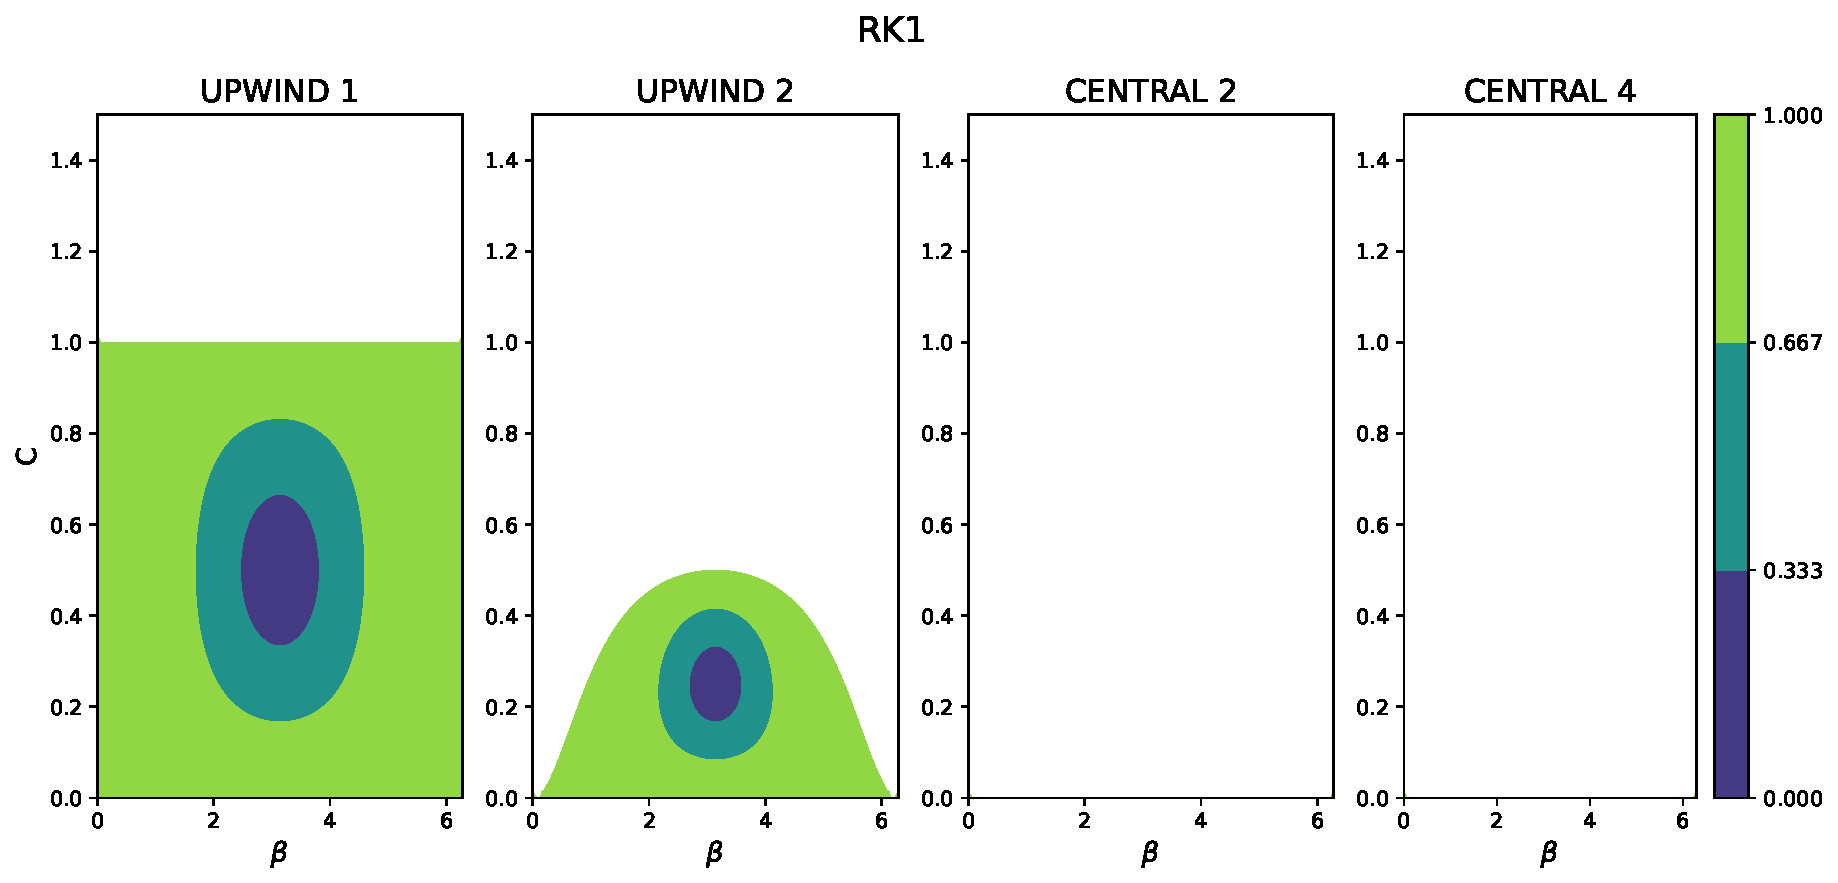
\includegraphics[width=0.8\linewidth]{./vn_rk1.pdf} % Adjust the width as necessary
    \caption{Amplification factor magnitude for the first-order Runge Kutta scheme.}
    \label{fig:vn_rk1} % For referencing the figure elsewhere in your document
\end{figure}

\begin{figure}[htbp]
    \centering
    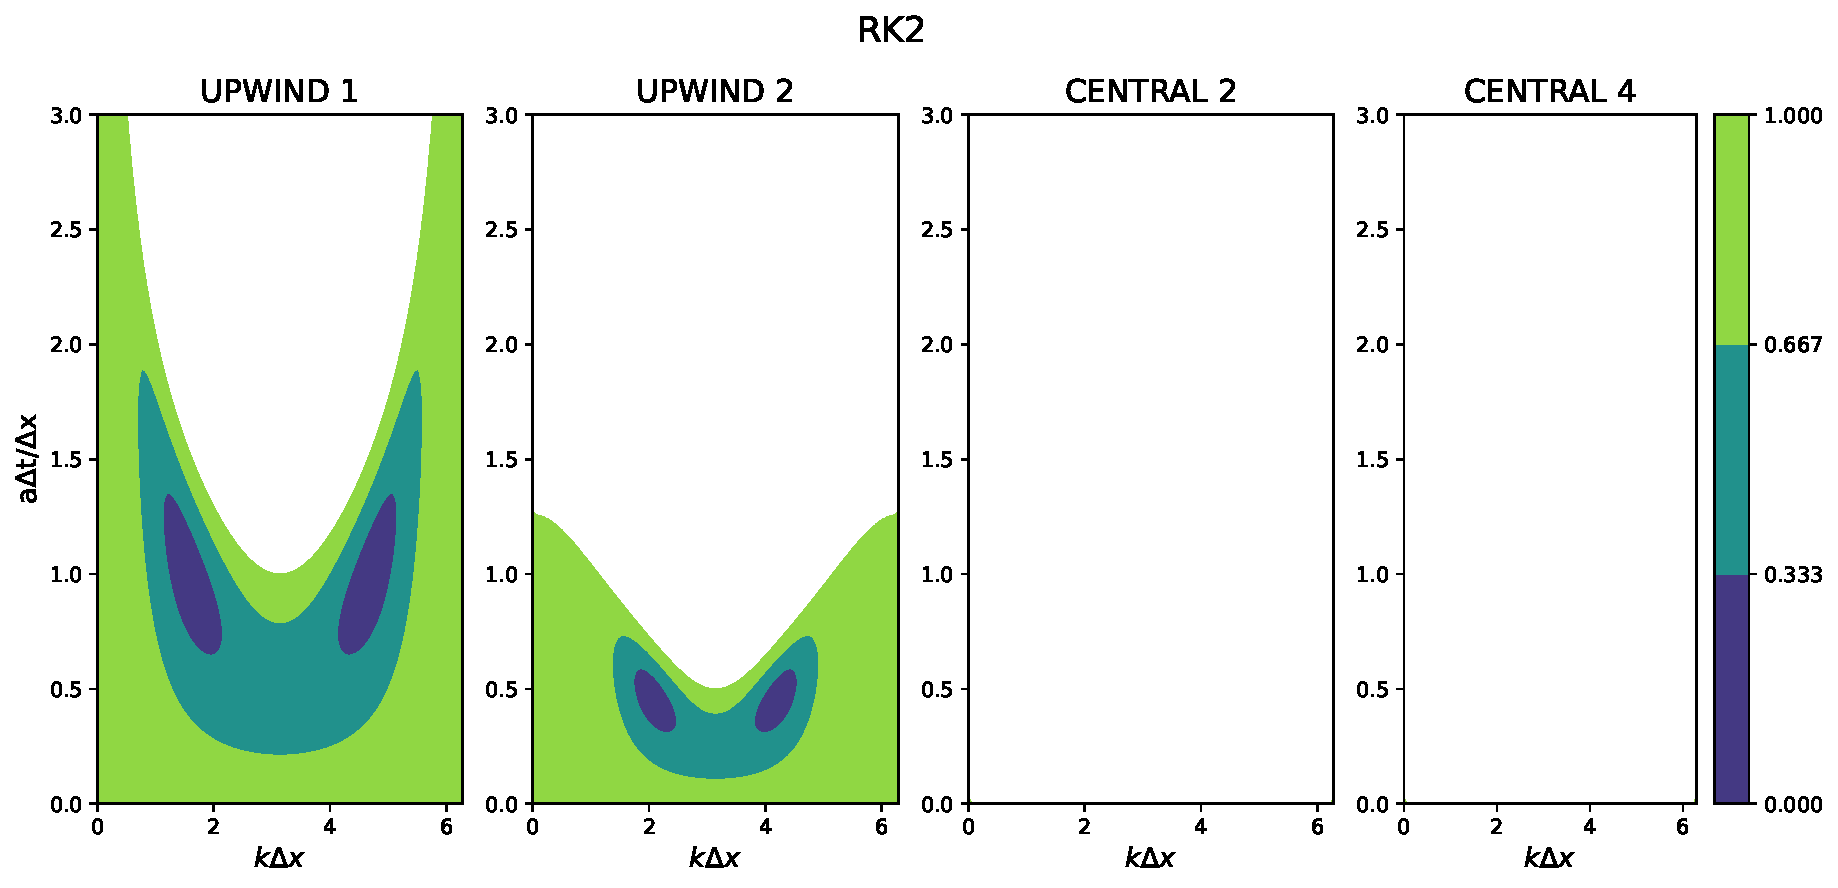
\includegraphics[width=0.8\linewidth]{./vn_rk2.pdf} % Adjust the width as necessary
    \caption{Amplification factor magnitude for the second-order Runge Kutta scheme.}
    \label{fig:vn_rk2} % For referencing the figure elsewhere in your document
\end{figure}

\begin{figure}[htbp]
    \centering
    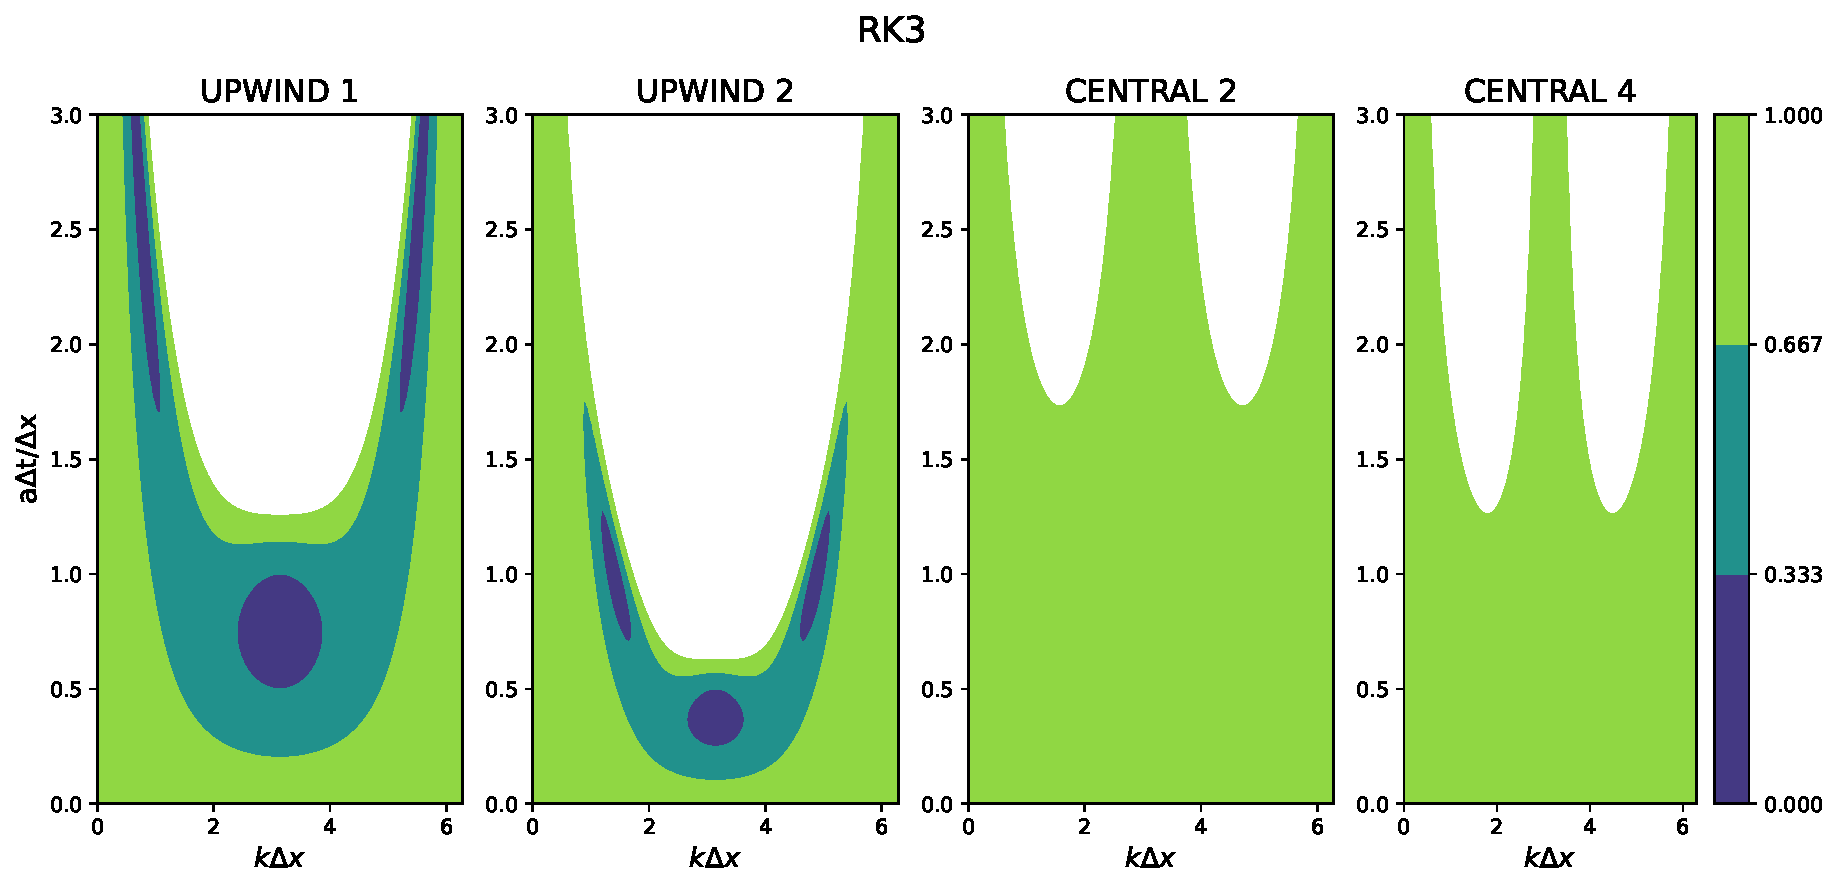
\includegraphics[width=0.8\linewidth]{./vn_rk3.pdf} % Adjust the width as necessary
    \caption{Amplification factor magnitude for the third-order Runge Kutta scheme.}
    \label{fig:vn_rk3} % For referencing the figure elsewhere in your document
\end{figure}

\begin{figure}[htbp]
    \centering
    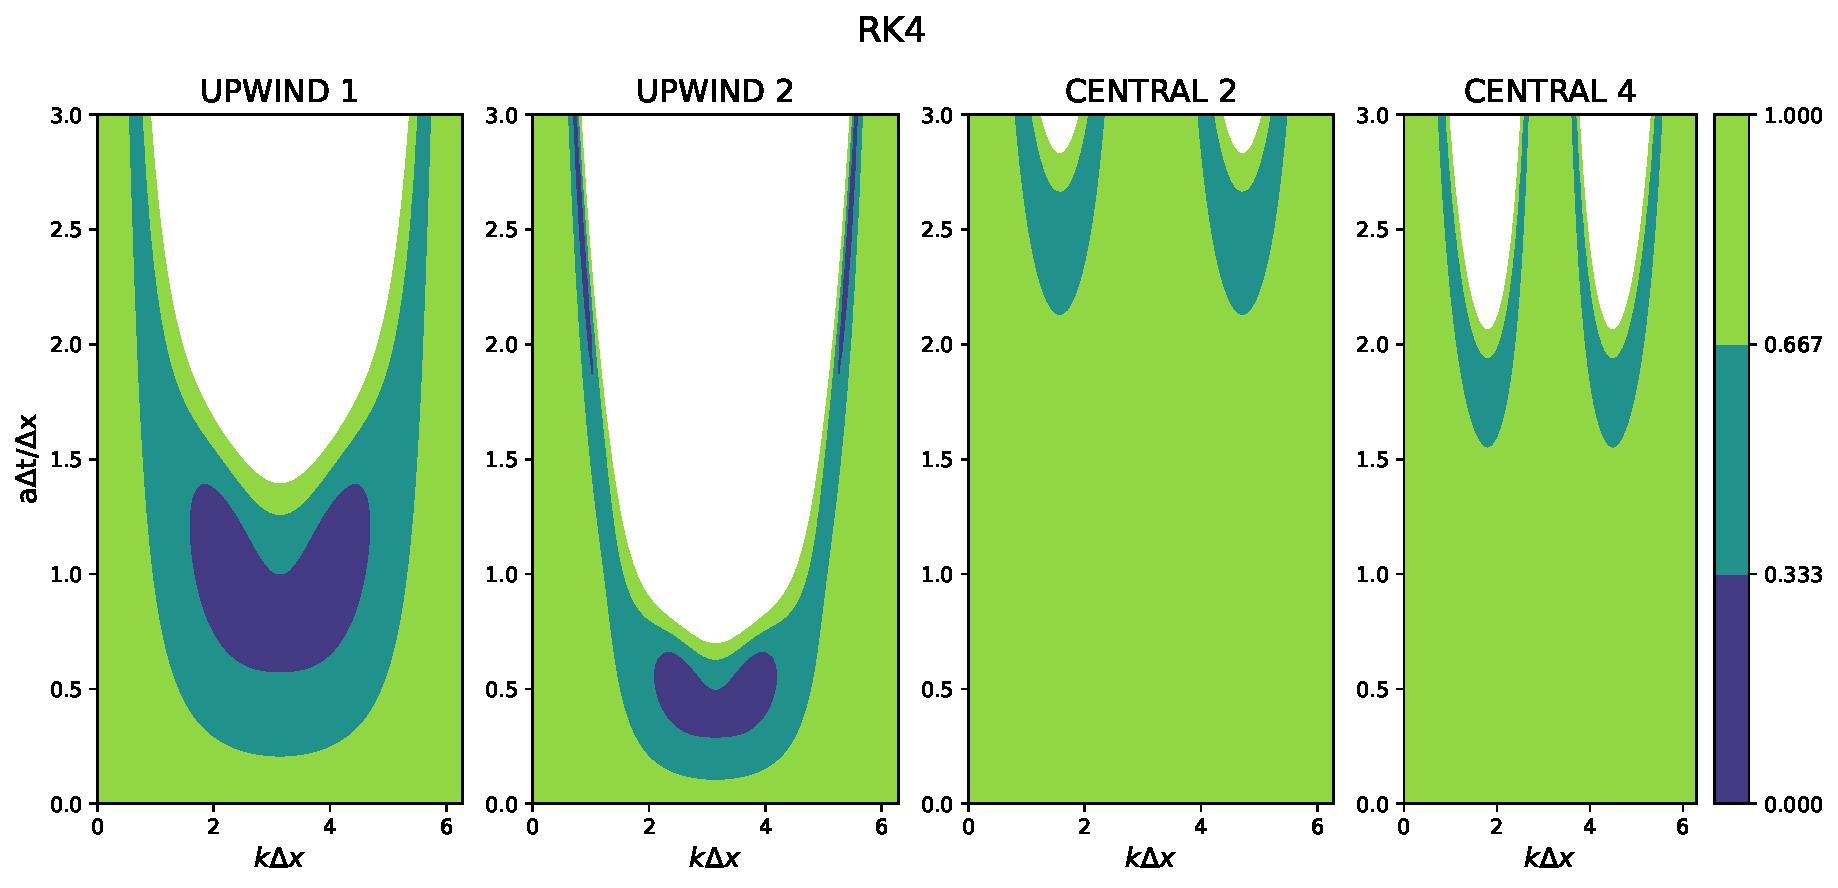
\includegraphics[width=0.8\linewidth]{./vn_rk4.pdf} % Adjust the width as necessary
    \caption{Amplification factor magnitude for the fourth-order Runge Kutta scheme.}
    \label{fig:vn_rk4} % For referencing the figure elsewhere in your document
\end{figure}






\bibliographystyle{apalike}
\bibliography{initialization.bib}

\end{document}